\documentclass[11pt]{article}
\usepackage[margin=1in]{geometry}
\usepackage{amsmath, amssymb}
\usepackage{graphicx}
\usepackage{booktabs}
\usepackage{hyperref}
\usepackage{setspace}
\usepackage{listings}
\usepackage{color}
\usepackage{tikz}
\usetikzlibrary{shapes.geometric, arrows, positioning, calc}

\definecolor{codegreen}{rgb}{0,0.6,0}
\definecolor{codegray}{rgb}{0.5,0.5,0.5}
\definecolor{codepurple}{rgb}{0.58,0,0.82}
\definecolor{backcolour}{rgb}{0.95,0.95,0.92}

\lstset{
    backgroundcolor=\color{backcolour},   
    commentstyle=\color{codegreen},
    keywordstyle=\color{codepurple},
    numberstyle=\tiny\color{codegray},
    stringstyle=\color{codepurple},
    basicstyle=\ttfamily\footnotesize,
    breakatwhitespace=false,         
    breaklines=true,                 
    captionpos=b,                    
    keepspaces=true,                 
    numbers=left,                    
    numbersep=5pt,                  
    showspaces=false,                
    showstringspaces=false,
    showtabs=false,                  
    tabsize=2
}

\title{Quant-Alpha Pipeline: Multi-Stage Residual Correction Architecture \\ \large Technical Documentation for Systematic Trading}
\author{Quantitative Research Team}
\date{\today}

\begin{document}

\maketitle
\tableofcontents
\newpage

\section{Introduction}
This document details a sophisticated two-stage forecasting pipeline designed for cross-sectional return prediction in equity markets. The architecture utilizes a baseline Gradient Boosted Decision Tree (GBDT) followed by parallel, decoupled residual correctors utilizing regime-inference (HMM) and sequence-modeling (Transformer) paradigms.

\section{Data Engineering \& Preprocessing Protocol}

\subsection{Data Cleaning and Imputation}
The raw company-month panels undergo a rigorous cleaning cycle to ensure signal integrity:
\begin{enumerate}
    \item \textbf{Infinite Value Suppression:} All instances of $\pm \infty$ are treated as missing values (NaN).
    \item \textbf{Missingness Encoding:} For every numeric feature $x_j$, a binary indicator feature $x_{j, \text{miss}} \in \{0, 1\}$ is generated to allow the model to learn specific biases associated with missing data reports.
    \item \textbf{Median Imputation:} Remaining NaNs are filled with the historical median of that specific feature. If a feature is entirely NaN for a company, it is initialized to 0.0 to maintain matrix dimensionality.
    \item \textbf{Target Transformation:} The target variable $y$ (\texttt{monthly\_gross\_return}) is log-transformed to stabilize variance: $\tilde{y} = \ln(y)$.
\end{enumerate}

\subsection{Feature Engineering: Generating Dynamic Signals}
Our pipeline engineers 493 unique features to capture cross-sectional and time-series alpha:
\begin{itemize}
    \item \textbf{Lagged Features:} Historical values for all fundamental features are generated for $L \in \{1, 2, 3, 6\}$ months to capture delayed market reactions.
    \item \textbf{Rolling Statistics:} Moving averages and standard deviations are computed over 3-month and 6-month windows:
    \[ \text{RollMean}_W = \frac{1}{W} \sum_{i=0}^{W-1} x_{t-i}, \quad \text{RollStd}_W = \sqrt{\frac{\sum (x_{t-i} - \bar{x})^2}{W-1}} \]
    \item \textbf{Return Momentum \& Volatility:} Calculated directly from the target return stream over 3 and 6 months to act as the primary inputs for regime detection.
\end{itemize}

\subsection{Categorical Variable Selection}
To capture structural differences across equity clusters, we utilize six primary categorical features, treated as ordered target statistics within the CatBoost framework:
\begin{enumerate}
    \item \textbf{Size\_Label}: Company market capitalization deciles.
    \item \textbf{BM\_Label}: Book-to-Market ratio deciles (Value vs. Growth).
    \item \textbf{OpProf\_Label}: Operating Profitability clusters.
    \item \textbf{Inv\_Label}: Investment intensity bins.
    \item \textbf{Mom\_Label}: Cross-sectional momentum deciles.
    \item \textbf{Quarter}: Seasonal temporal indicators (1, 2, 3, 4).
\end{enumerate}

\subsection{Preprocessing Pipeline Visualization}

\begin{figure}[h]
\centering
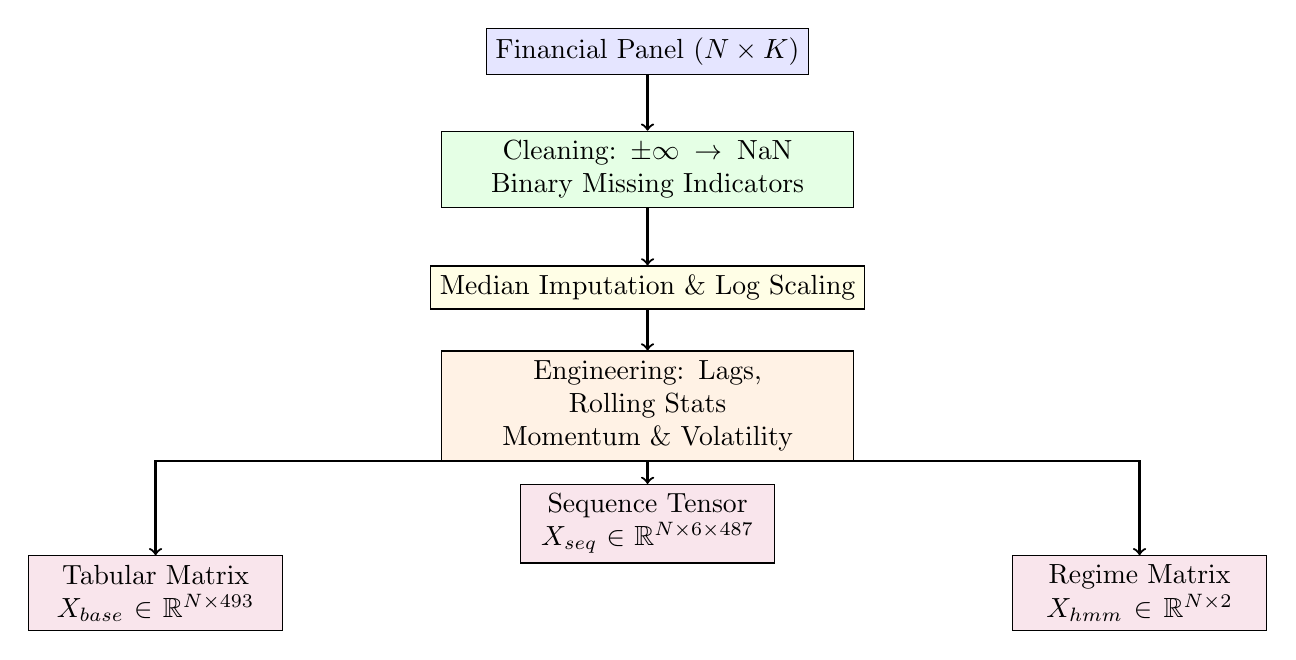
\begin{tikzpicture}[node distance=1.5cm, auto]
    \node (raw) [draw, rectangle, fill=blue!10] {Financial Panel ($N \times K$)};
    \node (clean) [draw, rectangle, below of=raw, fill=green!10, text width=5cm, align=center] {Cleaning: $\pm \infty \to \text{NaN}$ \\ Binary Missing Indicators};
    \node (imp) [draw, rectangle, below of=clean, fill=yellow!10] {Median Imputation \& Log Scaling};
    \node (eng) [draw, rectangle, below of=imp, fill=orange!10, text width=5cm, align=center] {Engineering: Lags, Rolling Stats \\ Momentum \& Volatility};
    
    \node (base) [draw, rectangle, below left=1.2cm and 2cm of eng, fill=purple!10, text width=3cm, align=center] {Tabular Matrix \\ $X_{base} \in \mathbb{R}^{N \times 493}$};
    \node (seq) [draw, rectangle, below of=eng, fill=purple!10, text width=3cm, align=center] {Sequence Tensor \\ $X_{seq} \in \mathbb{R}^{N \times 6 \times 487}$};
    \node (hmm) [draw, rectangle, below right=1.2cm and 2cm of eng, fill=purple!10, text width=3cm, align=center] {Regime Matrix \\ $X_{hmm} \in \mathbb{R}^{N \times 2}$};

    \draw [->, thick] (raw) -- (clean);
    \draw [->, thick] (clean) -- (imp);
    \draw [->, thick] (imp) -- (eng);
    \draw [->, thick] (eng.south) -| (base.north);
    \draw [->, thick] (eng.south) -- (seq.north);
    \draw [->, thick] (eng.south) -| (hmm.north);
\end{tikzpicture}
\caption{Systematic flow from raw panels to model-specific input tensors.}
\end{figure}

\section{Chronological Isolation: Training \& Evaluation Splits}

To prevent \textbf{Look-Ahead Bias}, we enforce a strict temporal separation. No model is allowed to see data from a future period during its respective training phase.

\begin{table}[h]
\centering
\begin{tabular}{lll}
\toprule
\textbf{Split Phase} & \textbf{Date Range} & \textbf{Purpose} \\
\midrule
\textbf{Training} & 2001-05 to 2020-12 & CatBoost Baseline Fit \\
\textbf{Validation} & 2021-01 to 2021-12 & Residual Correction Training (HMM/Transformer) \\
\textbf{Gap Buffer} & 2022-01 to 2022-06 & Temporal Isolation Buffer \\
\textbf{Test/Holdout} & 2022-07 to 2025-03 & Out-of-Sample Performance Evaluation \\
\bottomrule
\end{tabular}
\caption{The 4-stage chronological split strategy.}
\end{table}

\subsection{Decoupled Training Regimen}
Correctors are trained \textit{exclusively} on residuals generated by the frozen base model on the 2021 Validation period. This ensures that the HMM and Transformer learn to correct structural \textit{out-of-sample} errors rather than overfitting to the base model's training memorization.

\section{Architecture Details}

\subsection{Baseline Predictor: CatBoost GBDT}
The baseline regressor utilizes oblivious decision trees to establish a fundamental return forecast. 

\subsection{Regime-Aware Correction (Gaussian HMM)}
The HMM models latent market states $S_t$ based on $\sigma$ and $\Delta P$. It computes $\hat{r} = \mathbb{E}[r | S_t]$, adding a structural mean-correction to the CatBoost output.

\begin{figure}[h]
\centering
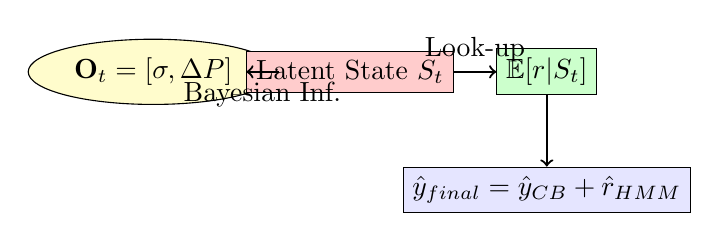
\begin{tikzpicture}[node distance=2.5cm, auto]
    \node (obs) [draw, ellipse, fill=yellow!20] {$\mathbf{O}_t = [\sigma, \Delta P]$};
    \node (hidden) [draw, rectangle, right of=obs, fill=red!20] {Latent State $S_t$};
    \node (map) [draw, rectangle, right of=hidden, fill=green!20] {$\mathbb{E}[r | S_t]$};
    \node (corr) [draw, rectangle, below of=map, node distance=1.5cm, fill=blue!10] {$\hat{y}_{final} = \hat{y}_{CB} + \hat{r}_{HMM}$};

    \draw [->, thick] (obs) -- node {Bayesian Inf.} (hidden);
    \draw [->, thick] (hidden) -- node {Look-up} (map);
    \draw [->, thick] (map) -- (corr);
\end{tikzpicture}
\caption{HMM-based regime mapping for structural bias correction.}
\end{figure}

\subsubsection{HMM Training Procedure}
The model is trained on the 2021 Validation set using the \textbf{Baum-Welch Algorithm} (Expectation-Maximization). 
\begin{itemize}
    \item \textbf{Transition Matrix ($A$):} Learns the probability $P(S_t | S_{t-1})$ of the market shifting moods.
    \item \textbf{Emission Parameters ($\mu, \Sigma$):} Fits a Gaussian distribution to the Volatility and Momentum signals for each state.
    \item \textbf{Residual Mapping:} After training, we run the model over the validation set to infer states for every data point and calculate the historical mean residual for each of the 3 regimes.
\end{itemize}

\subsubsection{HMM Inference Step}
During the test phase, for a given company $i$ at month $t$:
\begin{enumerate}
    \item We extract $[\sigma_{i,t}, \Delta P_{i,t}]$.
    \item We calculate the posterior probability $P(S_t = k | \mathbf{O}_t)$ using the \textbf{Forward Algorithm}.
    \item We select the state $k$ with the maximum probability.
    \item The final prediction is adjusted by the pre-calculated mean residual for state $k$.
\end{enumerate}

\subsection{Deep Sequence Correction (Transformer)}
The Transformer employs Multi-Head Self-Attention to model the residual term $\hat{r}_t$ over a 6-month trailing window. \textit{Note: This implementation does not utilize positional encoding, treating the sequence as a chronologically-bound set of snapshots.}

\begin{figure}[h]
\centering
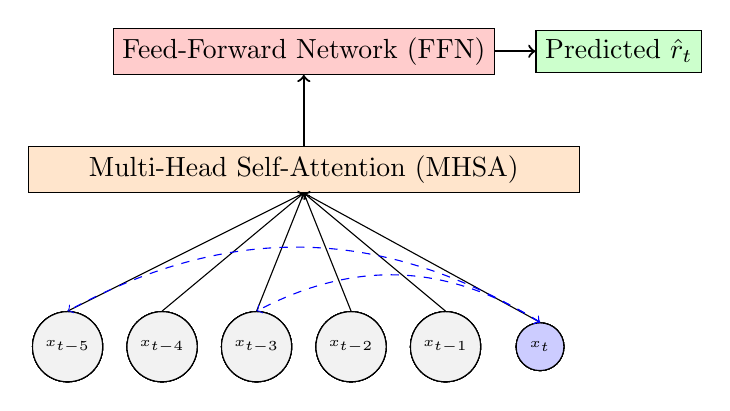
\begin{tikzpicture}[node distance=1.2cm, auto]
    \foreach \i in {1,...,6} {
        \node (m1) at (0,0) [draw, circle, fill=gray!10] {\tiny $x_{t-5}$};
        \node (m2) at (1.2,0) [draw, circle, fill=gray!10] {\tiny $x_{t-4}$};
        \node (m3) at (2.4,0) [draw, circle, fill=gray!10] {\tiny $x_{t-3}$};
        \node (m4) at (3.6,0) [draw, circle, fill=gray!10] {\tiny $x_{t-2}$};
        \node (m5) at (4.8,0) [draw, circle, fill=gray!10] {\tiny $x_{t-1}$};
        \node (m6) at (6.0,0) [draw, circle, fill=blue!20] {\tiny $x_{t}$};
    }

    \node (att) [draw, rectangle, above=1.5cm of m3, xshift=0.6cm, fill=orange!20, minimum width=7cm] {Multi-Head Self-Attention (MHSA)};
    \node (head) [draw, rectangle, above of=att, node distance=1.5cm, fill=red!20] {Feed-Forward Network (FFN)};
    \node (out) [draw, rectangle, right of=head, node distance=4cm, fill=green!20] {Predicted $\hat{r}_t$};

    \foreach \i in {1,...,6} { \draw [->] (m\i.north) -- (att.south); }
    \draw [<->, dashed, blue] (m6.north) to [bend right=30] (m3.north);
    \draw [<->, dashed, blue] (m6.north) to [bend right=30] (m1.north);
    \draw [->, thick] (att) -- (head);
    \draw [->, thick] (head) -- (out);
\end{tikzpicture}
\caption{Transformer architecture for sequence-based residual forecasting.}
\end{figure}

\subsubsection{Transformer Training Procedure}
The Transformer is trained to minimize the MSE of the 2021 validation residuals:
\begin{itemize}
    \item \textbf{Optimization:} Adam optimizer with $\eta = 1e-4$.
    \item \textbf{Feature Compression:} A linear embedding layer maps the 487 input features into a 64-dimensional latent space before attention.
    \item \textbf{Global Pooling:} After the MHSA layers, we apply a temporal mean-pooling across the 6 months to create a fixed-length vector for the final regression head.
\end{itemize}

\subsubsection{Transformer Inference Step}
For a company $i$ at month $t$:
\begin{enumerate}
    \item A sliding window of the previous 6 months $[x_{t-5}, \dots, x_t]$ is extracted.
    \item The sequence is passed through the pre-trained Transformer layers.
    \item The model outputs a predicted correction value $\hat{r}_t$.
    \item This correction is added to the base CatBoost prediction.
\end{enumerate}

\end{document}
